% =====================================================================
%  Paper 4 — supplementary material. Build after scripts/paper4_figures.py:  tectonic -X compile paper4_supplement.tex
%  Every number is a macro from figs4/numbers4.tex or a cell of a generated table; none is typed here.
% =====================================================================
\documentclass[journal]{IEEEtran}
\usepackage{graphicx,booktabs,amsmath,amssymb,xcolor,url,array}
\graphicspath{{figs4/}{figs3/}{figs2/}}
\newcommand{\FILL}[1]{\textcolor{red}{\textbf{[FILL: #1]}}}
\IEEEoverridecommandlockouts
\usepackage{iftex}\ifXeTeX\usepackage{fontspec}\setmainfont{texgyretermes}[Extension=.otf,UprightFont=*-regular,BoldFont=*-bold,ItalicFont=*-italic,BoldItalicFont=*-bolditalic]\fi
\raggedbottom
% generated by scripts/paper4_figures.py (includes every macro of scripts/paper3_figures.py); do not edit
\newcommand{\selArm}{B}
\newcommand{\BcvQ}{0.825}
\newcommand{\BcvQci}{[0.737, 0.911]}
\newcommand{\BdevQ}{0.756}
\newcommand{\BdevQci}{[0.679, 0.821]}
\newcommand{\BlosoQ}{0.834}
\newcommand{\nArms}{9}
\newcommand{\nTrained}{7}
\newcommand{\poolImages}{6{,}700}
\newcommand{\poolInfants}{1{,}528}
\newcommand{\poolSources}{3}
\newcommand{\dupExcl}{14}
\newcommand{\cvScored}{6{,}686}
\newcommand{\devImages}{663}
\newcommand{\devEyes}{230}
\newcommand{\devInfants}{116}
\newcommand{\lockedImages}{661}
\newcommand{\lockedEyes}{230}
\newcommand{\nReps}{2{,}000}
\newcommand{\bootSeed}{42}
\newcommand{\cvLists}{2}
\newcommand{\devLists}{10}
\newcommand{\seedA}{42}
\newcommand{\seedB}{1337}
\newcommand{\marginCV}{0.010}
\newcommand{\marginLOSO}{0.010}
\newcommand{\nAmend}{5}
\newcommand{\lastAmendDate}{2026-10-31}
\newcommand{\protoCommit}{ac33f29}
\newcommand{\protoDate}{2026-10-20}
\newcommand{\nArch}{11}
\newcommand{\nArmsAll}{20}
\newcommand{\transArms}{F}
\newcommand{\nPairs}{12}
\newcommand{\nRuns}{10}
\newcommand{\shortcutAUC}{0.911}
\newcommand{\lockedOpened}{2026-08-18}
\newcommand{\nSevereFrom}{3}
\newcommand{\gpu}{Tesla T4}
\newcommand{\mateN}{3{,}141}
\newcommand{\mateMatched}{2{,}964}
\newcommand{\mateUnmatched}{177}
\newcommand{\mateSrcRopvl}{1{,}438}
\newcommand{\mateSrcMultiview}{896}
\newcommand{\mateSrcShenzhen}{630}
\newcommand{\mateDevTrain}{390}
\newcommand{\mateLockedTrain}{331}
\newcommand{\matePoolTrain}{1{,}647}
\newcommand{\mateTrain}{2{,}512}
\newcommand{\mateVal}{314}
\newcommand{\mateTest}{315}
\newcommand{\mateMLTest}{629}
\newcommand{\mateLeakTest}{73\%}
\newcommand{\mateLeakVal}{73\%}
\newcommand{\mateLeakMV}{99\%}
\newcommand{\mateMLFeat}{428}
\newcommand{\mateMLBest}{SVM (RBF)}
\newcommand{\mateMLAcc}{0.585}
\newcommand{\mateMLQ}{0.547}
\newcommand{\mateCNNBest}{resnest50d}
\newcommand{\mateCNNAcc}{0.835}
\newcommand{\mateCNNQ}{0.898}
\newcommand{\mateCNNEnsAcc}{0.825}
\newcommand{\mateCNNDiverged}{convnext\_tiny}
\newcommand{\mateCNNDivergedAcc}{0.530}
\newcommand{\mateFMlo}{0.787}
\newcommand{\mateFMhi}{0.832}
\newcommand{\mateFMmean}{0.814}
\newcommand{\mateFMsd}{0.023}
\newcommand{\mateFMtrainable}{6.30}
\newcommand{\mateFMtotal}{309.7}
\newcommand{\mateFMbaseAcc}{0.825}
\newcommand{\mateFMbaseTrainable}{2.37}
\newcommand{\mateFMcomboAcc}{0.651}
\newcommand{\mateEnsAcc}{0.844}
\newcommand{\mateEnsQ}{0.900}
\newcommand{\mateBestAcc}{0.860}
\newcommand{\mateBestQ}{0.908}
\newcommand{\mateBestAUC}{0.972}
\newcommand{\mateBestN}{7}
\newcommand{\mateBestAccci}{[0.820, 0.896]}
\newcommand{\mateCIkind}{infant-clustered bootstrap}
\newcommand{\mateHalfWidth}{4}
\newcommand{\mateCommit}{424ad77}
\newcommand{\nMateSeries}{33}
\newcommand{\mateDate}{2026-11-07}
\newcommand{\acqImages}{13{,}037}
\newcommand{\acqSources}{11}
\newcommand{\acqExcluded}{2{,}610}
\newcommand{\stageLabelled}{10{,}427}
\newcommand{\stageInfants}{2{,}015}
\newcommand{\sixElig}{8{,}024}
\newcommand{\sixInfants}{1{,}760}
\newcommand{\exclOther}{1{,}295}
\newcommand{\exclTreated}{1{,}063}
\newcommand{\exclStageZero}{45}
\newcommand{\exclSix}{2{,}403}
\newcommand{\trainEligible}{3{,}112}
\newcommand{\vfourTrain}{3{,}083}
\newcommand{\poolValOnly}{3{,}588}
\newcommand{\capNormal}{2}
\newcommand{\capOther}{20}
\newcommand{\rawMultiview}{1{,}324}
\newcommand{\rawMultiviewInf}{232}
\newcommand{\rawOstrava}{6{,}004}
\newcommand{\rawOstravaInf}{187}
\newcommand{\rawRopvl}{2{,}020}
\newcommand{\rawRopvlInf}{1{,}116}
\newcommand{\rawShenzhen}{1{,}079}
\newcommand{\rawShenzhenInf}{480}
\newcommand{\poolOstrava}{4{,}285}
\newcommand{\poolOstravaInf}{148}
\newcommand{\perInfantOstrava}{29.0}
\newcommand{\poolRopvl}{1{,}675}
\newcommand{\poolRopvlInf}{983}
\newcommand{\perInfantRopvl}{1.7}
\newcommand{\poolShenzhen}{740}
\newcommand{\poolShenzhenInf}{397}
\newcommand{\perInfantShenzhen}{1.9}
\newcommand{\siteDecodable}{0.997}
\newcommand{\metaFloorCV}{0.187}
\newcommand{\metaFloorDev}{0.062}
\newcommand{\dupExact}{0}
\newcommand{\dupNear}{0}
\newcommand{\humanInterKappa}{0.24}
\newcommand{\humanIntraKappa}{0.56}
\newcommand{\humanDisagree}{40\%}
\newcommand{\vTwoKappaU}{0.655}
\newcommand{\BkappaU}{0.637}
\newcommand{\BdevKappaU}{0.527}
\newcommand{\vOneAcc}{0.733}
\newcommand{\vOneFone}{0.706}
\newcommand{\sweepAUC}{0.927}
\newcommand{\sweepValAUC}{0.842}
\newcommand{\vTwoCvQsix}{0.761}
\newcommand{\vTwoCvAcc}{0.786}
\newcommand{\vTwoLockedImgQ}{0.473}
\newcommand{\vTwoLockedEyeQ}{0.813}
\newcommand{\vTwoLockedEyeAcc}{0.646}
\newcommand{\vTwoGapMin}{0.32}
\newcommand{\vTwoGapMax}{0.34}
\newcommand{\sweepSelAUC}{0.964}
\newcommand{\sweepArchs}{5}
\newcommand{\mateMLReportAcc}{0.568}
\newcommand{\BkappaUpooled}{0.635}
\newcommand{\BdevKappaUpooled}{0.524}
\newcommand{\BthrPct}{98.94\%}
\newcommand{\BcvSens}{0.900}
\newcommand{\BcvSpec}{0.996}
\newcommand{\BdevSens}{0.656}
\newcommand{\BdevSpec}{1.000}
\newcommand{\BdevSevereSens}{0.927}
\newcommand{\BdevECE}{0.157}
\newcommand{\BdevRecNormal}{0.948}
\newcommand{\BcvRecNormal}{0.909}
\newcommand{\BdevRecStageOne}{0.510}
\newcommand{\BcvRecStageOne}{0.583}
\newcommand{\BdevRecStageTwo}{0.546}
\newcommand{\BcvRecStageTwo}{0.561}
\newcommand{\BdevRecStageThree}{0.566}
\newcommand{\BcvRecStageThree}{0.722}
\newcommand{\BdevRecStageFourFive}{0.580}
\newcommand{\BcvRecStageFourFive}{0.882}
\newcommand{\BdevRecArop}{0.700}
\newcommand{\BcvRecArop}{0.389}
\newcommand{\BdevAcc}{0.630}
\newcommand{\BdevMF}{0.566}
\newcommand{\BdevAUC}{0.937}
\newcommand{\BcvAcc}{0.766}
\newcommand{\BcvAUC}{0.979}
\newcommand{\BfoldMinutes}{33}
\newcommand{\nGenerations}{4}
\newcommand{\cvDiffAC}{−0.022}
\newcommand{\cvDiffACci}{[$-$0.052, +0.008]}
\newcommand{\cvDiffAB}{−0.031}
\newcommand{\cvDiffABci}{[$-$0.077, +0.015]}
\newcommand{\cvDiffBC}{+0.009}
\newcommand{\cvDiffBCci}{[$-$0.018, +0.027]}
\newcommand{\cvDiffEC}{+0.005}
\newcommand{\cvDiffECci}{[$-$0.007, +0.019]}
\newcommand{\cvDiffEA}{+0.026}
\newcommand{\cvDiffEAci}{[+0.008, +0.046]}
\newcommand{\cvDiffDA}{+0.002}
\newcommand{\cvDiffDAci}{[$-$0.057, +0.046]}
\newcommand{\cvDiffDB}{−0.029}
\newcommand{\cvDiffDBci}{[$-$0.051, +0.003]}
\newcommand{\cvDiffFB}{−0.014}
\newcommand{\cvDiffFBci}{[$-$0.035, +0.008]}
\newcommand{\cvDiffGB}{−0.011}
\newcommand{\cvDiffGBci}{[$-$0.036, +0.012]}
\newcommand{\cvDiffHB}{−0.013}
\newcommand{\cvDiffHBci}{[$-$0.031, +0.009]}
\newcommand{\cvDiffIB}{−0.004}
\newcommand{\cvDiffIBci}{[$-$0.015, +0.007]}
\newcommand{\cvDiffIH}{+0.009}
\newcommand{\cvDiffIHci}{[$-$0.007, +0.020]}
\newcommand{\devDiffAC}{+0.014}
\newcommand{\devDiffACci}{[$-$0.012, +0.048]}
\newcommand{\devDiffAB}{+0.019}
\newcommand{\devDiffABci}{[+0.000, +0.041]}
\newcommand{\devDiffBC}{−0.004}
\newcommand{\devDiffBCci}{[$-$0.038, +0.030]}
\newcommand{\devDiffEC}{+0.010}
\newcommand{\devDiffECci}{[$-$0.012, +0.040]}
\newcommand{\devDiffEA}{−0.004}
\newcommand{\devDiffEAci}{[$-$0.020, +0.008]}
\newcommand{\devDiffDA}{−0.028}
\newcommand{\devDiffDAci}{[$-$0.048, $-$0.011]}
\newcommand{\devDiffDB}{−0.009}
\newcommand{\devDiffDBci}{[$-$0.019, +0.001]}
\newcommand{\devDiffFB}{−0.012}
\newcommand{\devDiffFBci}{[$-$0.022, $-$0.002]}
\newcommand{\devDiffGB}{+0.012}
\newcommand{\devDiffGBci}{[$-$0.006, +0.032]}
\newcommand{\devDiffHB}{−0.006}
\newcommand{\devDiffHBci}{[$-$0.015, +0.003]}
\newcommand{\devDiffIB}{+0.020}
\newcommand{\devDiffIBci}{[+0.003, +0.041]}
\newcommand{\devDiffIH}{+0.026}
\newcommand{\devDiffIHci}{[+0.006, +0.046]}
\newcommand{\BostravaQ}{0.701}
\newcommand{\BropvlQ}{0.930}
\newcommand{\BshenzhenQ}{0.967}
\newcommand{\DostravaQ}{0.846}
\newcommand{\DropvlQ}{0.925}
\newcommand{\DshenzhenQ}{0.967}
\newcommand{\CostravaQ}{0.775}
\newcommand{\CropvlQ}{0.921}
\newcommand{\CshenzhenQ}{0.967}
\newcommand{\cvQAsA}{0.797}
\newcommand{\devQAsA}{0.772}
\newcommand{\cvQAsB}{0.791}
\newcommand{\devQAsB}{0.776}
\newcommand{\cvQBsA}{0.835}
\newcommand{\devQBsA}{0.754}
\newcommand{\cvQBsB}{0.815}
\newcommand{\devQBsB}{0.757}
\newcommand{\cvQCsA}{0.819}
\newcommand{\devQCsA}{0.756}
\newcommand{\cvQCsB}{0.813}
\newcommand{\devQCsB}{0.764}
\newcommand{\mdd}{0.08}
\newcommand{\eqCvWithin}{12}
\newcommand{\eqCvZero}{11}
\newcommand{\eqCvTotal}{12}
\newcommand{\eqDevWithin}{12}
\newcommand{\eqDevZero}{7}
\newcommand{\eqDevTotal}{12}
\newcommand{\BcvQsix}{0.779}
\newcommand{\BostravaQci}{[0.490, 0.776]}
\newcommand{\BostravaQr}{0.701}
\newcommand{\BropvlQci}{[0.915, 0.943]}
\newcommand{\BropvlQr}{0.930}
\newcommand{\BshenzhenQci}{[0.958, 0.976]}
\newcommand{\BshenzhenQr}{0.967}
\newcommand{\CostravaQci}{[0.522, 0.876]}
\newcommand{\CostravaQr}{0.775}
\newcommand{\CropvlQci}{[0.902, 0.936]}
\newcommand{\CropvlQr}{0.921}
\newcommand{\CshenzhenQci}{[0.957, 0.975]}
\newcommand{\CshenzhenQr}{0.967}
\newcommand{\DostravaQci}{[0.692, 0.917]}
\newcommand{\DostravaQr}{0.846}
\newcommand{\DropvlQci}{[0.909, 0.939]}
\newcommand{\DropvlQr}{0.925}
\newcommand{\DshenzhenQci}{[0.954, 0.976]}
\newcommand{\DshenzhenQr}{0.967}
\newcommand{\devPhotosPerEyeMedian}{3}
\newcommand{\devPhotosPerEyeMin}{1}
\newcommand{\devPhotosPerEyeMax}{4}
\newcommand{\devEyesThreeViews}{186}
\newcommand{\devPhotosNormalMean}{2.94}
\newcommand{\devPhotosDiseasedMean}{2.87}
\newcommand{\devPhotosSevereMean}{2.94}
\newcommand{\BdevQens}{0.752}
\newcommand{\BdevQensci}{[0.671, 0.822]}
\newcommand{\BdevSensEns}{0.656}
\newcommand{\BdevSensEnsci}{[0.571, 0.740]}
\newcommand{\BdevSpecEns}{1.000}
\newcommand{\BdevSpecEnsci}{[1.000, 1.000]}
\newcommand{\BdevQthree}{0.782}
\newcommand{\BdevQthreeci}{[0.697, 0.849]}
\newcommand{\devEyesPos}{180}
\newcommand{\devEyesNeg}{50}
\newcommand{\vtServedEyeQ}{0.839}
\newcommand{\vtServedEyeQci}{[0.768, 0.890]}
\newcommand{\vtServedEyeAcc}{0.678}
\newcommand{\vtServedEyeMF}{0.616}
\newcommand{\vtServedImgQ}{0.493}
\newcommand{\vtServedImgAcc}{0.546}
\newcommand{\vtServedImgAUC}{0.835}
\newcommand{\vtStructParams}{20{,}512{,}600}
\newcommand{\vtDropPairs}{6{,}058}

\renewcommand{\arraystretch}{1.05}
\renewcommand{\thetable}{S\arabic{table}}
\renewcommand{\thefigure}{S\arabic{figure}}
\setcounter{topnumber}{4}\setcounter{dbltopnumber}{4}\setcounter{totalnumber}{8}
\renewcommand{\topfraction}{0.95}\renewcommand{\dbltopfraction}{0.95}\renewcommand{\textfraction}{0.05}

\title{Supplementary Material for ``Classical Learners, Convolutional Networks and Vision Transformers for ICROP-3 Staging of Retinopathy of Prematurity: An Audited Development across Four Public Cohorts''}
\author{Praharsh~Nagpure, \FILL{R. Bait full name}, \FILL{P. Rangnekar full name}, \FILL{Y. Shengale full name}, and \FILL{A. Kumar full name}}
\markboth{Supplementary material, November 2026}{Nagpure \MakeLowercase{\emph{et al.}}: Supplementary material}

\begin{document}
\maketitle

\section{Contents}
Tables~\ref{tab:funnel}--\ref{tab:matefm} and Figs.~\ref{fig:loso}--\ref{fig:webapp} hold the material referred to from the main text; Table~\ref{tab:claim} maps the CLAIM 2024 items to where each is reported. All of it is generated by \texttt{scripts/paper4\_figures.py} from the files named in the main text's Data and Code Availability statement.

\section{Data}
\begin{table*}[!t]
\caption{Acquisition cascade in numbers, and how the eligible photographs are used. Removed photographs at the training-eligible step stay in validation: every photograph of the pool is scored exactly once by the model that never trained on its infant.}
\label{tab:funnel}
\centering\scriptsize\setlength{\tabcolsep}{4pt}
\begin{tabular}{@{}lrrr>{\raggedright\arraybackslash}p{7.6cm}@{}}
\toprule
Step & Photos & Infants & Removed & Reason / note\\
\midrule
Acquired & 13{,}037 & -- & -- & 11 publicly released sources \\
Stage-labelled cohorts & 10{,}427 & 2{,}015 & 2{,}610 & no ICROP stage label (plus-only, segmentation sets), too small to fold, re-encoded duplicates \\
Six-class eligible & 8{,}024 & 1{,}760 & 2{,}403 & other pathology 1{,}295, treated 1{,}063, stage 0 45 \\
Cross-validation pool & 6{,}700 & 1{,}528 & -- & three cohorts; every photo in one validation fold \\
Training-eligible & 3{,}112 & 1{,}528 & 3{,}588 & per-infant caps: 2 normal, 20 per disease class; capped photos stay in validation \\
Held-out cohort, dev half & 663 & 116 & -- & 230 eyes; checks and every reported external number \\
Held-out cohort, locked half & 661 & 116 & -- & 230 eyes; opened once, Aug 2026, for the CNN generation \\
\bottomrule
\end{tabular}

\end{table*}

\begin{figure}[!t]
\centering
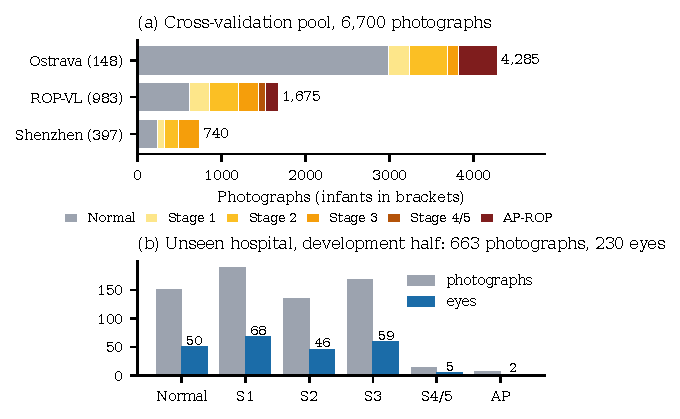
\includegraphics[width=\columnwidth]{fig_dataset.pdf}
\caption{Cross-validation pool by cohort and stage (a), and the held-out cohort's development half by stage (b): photographs and eyes.}
\label{fig:dataset}
\end{figure}

\begin{figure*}[!t]
\centering
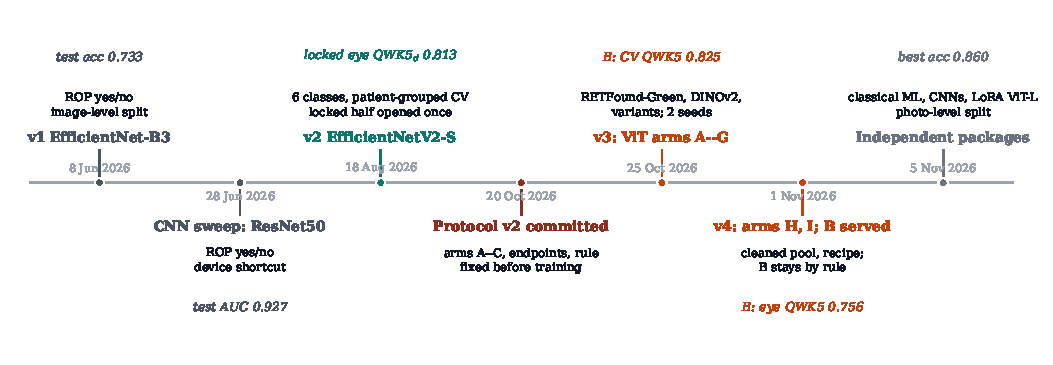
\includegraphics[width=\textwidth]{fig_timeline.pdf}
\caption{The development in time, with each generation's split type and its headline under its own protocol. Numbers across generations are not comparable (main text, Table~VII).}
\label{fig:timeline}
\end{figure*}

\section{Generation 1: convolutional networks}
\begin{table}[!t]
\caption{First model (June 2026): EfficientNet-B3, one shared model for binary ROP and diabetic retinopathy (DR), image-level split. P / R: precision / recall. Retired: image-level split and two diseases in one model.}
\label{tab:v1}
\centering\scriptsize\setlength{\tabcolsep}{2.0pt}
\begin{tabular}{@{}>{\raggedright\arraybackslash}p{1.45cm}rccccc@{}}
\toprule
Split & n & Acc. & mF1 & No ROP P / R & ROP P / R & ROP F1\\
\midrule
ROP val & 928 & 0.647 & 0.646 & 0.476 / 0.933 & 0.941 / 0.510 & 0.661 \\
ROP test & 1{,}502 & 0.733 & 0.731 & 0.644 / 0.913 & 0.891 / 0.585 & 0.706 \\
DR val, ep.\ 5 & -- & 0.719 & 0.497 & -- & -- & -- \\
\bottomrule
\end{tabular}

\end{table}

\begin{table}[!t]
\caption{June 2026 binary CNN sweep (ROP yes/no, Ostrava, sweep validation split; QWK$_2$: binary kappa) and, $^\ast$, the deployed ResNet50 on its own validation and test split. Inflated by the device shortcut: image size alone reached AUC \shortcutAUC{} on the same split.}
\label{tab:sweep}
\centering\scriptsize\setlength{\tabcolsep}{2.2pt}
\begin{tabular}{@{}lcccccc@{}}
\toprule
Architecture & Acc. & mF1 & QWK$_2$ & AUC & Params (M) & CPU ms\\
\midrule
efficientnet\_b0 & 0.758 & 0.757 & 0.525 & 0.867 & 4.01 & 56.2 \\
efficientnet\_v2\_s & 0.706 & 0.701 & 0.431 & 0.870 & 20.18 & 130.1 \\
mobilenet\_v3\_large & 0.744 & 0.743 & 0.500 & 0.857 & 4.2 & 34.4 \\
resnet50 & 0.886 & 0.882 & 0.766 & 0.964 & 23.51 & 157.2 \\
densenet121 & 0.764 & 0.764 & 0.537 & 0.887 & 6.96 & 136 \\
\midrule
resnet50$^\ast$ val & 0.747 & 0.740 & 0.499 & 0.842 & -- & -- \\
resnet50$^\ast$ test & 0.844 & 0.843 & 0.688 & 0.927 & -- & -- \\
\bottomrule
\end{tabular}

\end{table}

\section{Generation 2: vision transformers}
\begin{table*}[!t]
\caption{Recipe and cost of the transformer arms. Shared by every trained arm: circle-crop, letterbox, CLAHE; class-balanced cross-entropy; strong and site-randomizing augmentation; batch 16; AdamW; one-cycle cosine schedule; last-epoch weights. LLRD: layer-wise learning-rate decay; LS: label smoothing. Cost: mean over cross-validation folds and both seeds on Kaggle \gpu{} GPUs; C and E were not trained in this generation.}
\label{tab:recipe}
\centering\scriptsize\setlength{\tabcolsep}{3pt}
\begin{tabular}{@{}llcllcccc>{\raggedright\arraybackslash}p{6.2cm}cc@{}}
\toprule
Arm & Backbone & px & Norm. & Pool & Peak lr & LLRD & LS & Ep. & Differences from B's recipe & min/fold & img/s\\
\midrule
A & \texttt{retfound\_green} & 392 & half & v3 & 2e-4 & 0.8 & 0.05 & 20 & RETFound-Green weights & 32.1 & 38.6 \\
\textbf{B} & \texttt{dinov2\_s} & 392 & imagenet & v3 & 1e-4 & 0.8 & 0.05 & 20 & reference recipe & 33.3 & 31.9 \\
C & \texttt{effnetv2s} & 384 & imagenet & v3 & 3e-4 & -- & 0.05 & 20 & v2 flat softmax, natural sampler; saved predictions re-scored & -- & -- \\
D & \texttt{dinov2\_s} & 392 & imagenet & v3 & 1e-4 & 0.8 & 0.05 & 20 & LSE bag loss on Ostrava sessions, $K{=}8$, $\tau{=}1$ & 32.5 & 29.0 \\
E & -- & -- & -- & v3 & -- & -- & -- & -- & mean of A, B, C probabilities, matched by seed; no training & -- & -- \\
F$^\dagger$ & \texttt{dinov2\_s} & 392 & imagenet & v3 & 1e-4 & 0.8 & 0.05 & 20 & self-ensembling on unlabelled dev photos, EMA 0.99, conf.\ $\ge$0.9 & 61.7 & 14.2 \\
G & \texttt{dinov2\_s} & 518 & imagenet & v3 & 1e-4 & 0.8 & 0.05 & 20 & 518 px & 58.1 & 19.2 \\
H & \texttt{dinov2\_s} & 392 & imagenet & v4 & 1e-4 & 0.8 & 0.05 & 20 & v4 pool (per-device quality filter) & 34.1 & 31.2 \\
I & \texttt{dinov2\_s} & 392 & imagenet & v4 & 1e-4 & 0.8 & 0.1 & 20 & EMA weights 0.999; 1 head-only epoch; label smoothing 0.1; rot.\ $\pm$180$^\circ$, crop $\ge$0.85, gamma, noise, Fourier swap $p\,0.5$ & 34.8 & 32.1 \\
\bottomrule
\end{tabular}

\end{table*}

\begin{figure}[!t]
\centering
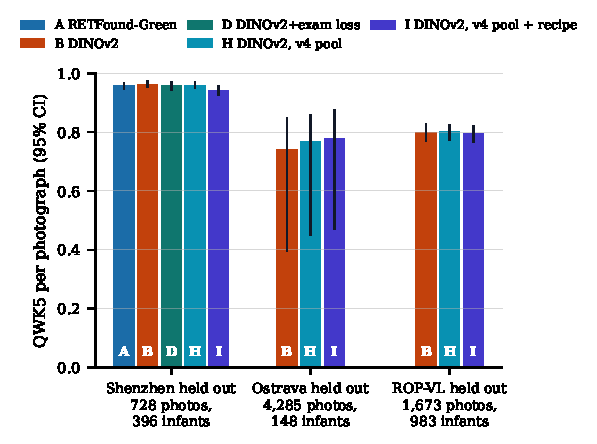
\includegraphics[width=\columnwidth]{fig_loso.pdf}
\caption{Leave-one-source-out folds: each model trains on two cohorts and scores every photograph of the third (both seeds pooled). Stage 4/5 exists only in ROP-VL, so that fold scores it untrained.}
\label{fig:loso}
\end{figure}

\begin{figure*}[!t]
\centering
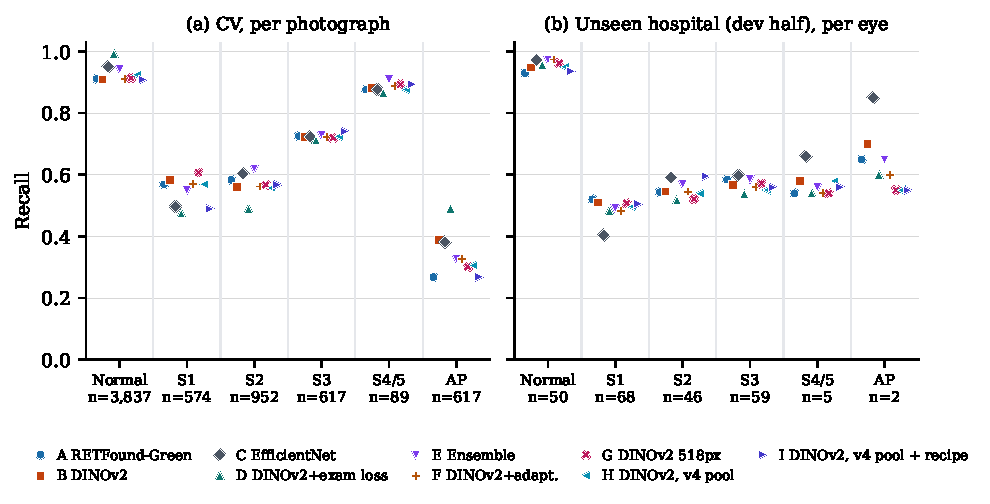
\includegraphics[width=\textwidth]{fig_stage_recall.pdf}
\caption{Recall per class, all transformer arms: (a) cross-validation per photograph; (b) held-out cohort per eye. n below each class: photographs (a), eyes (b). Arm identity by color and marker; the values are in the main text's per-class table.}
\label{fig:stage}
\end{figure*}

\begin{figure*}[!t]
\centering
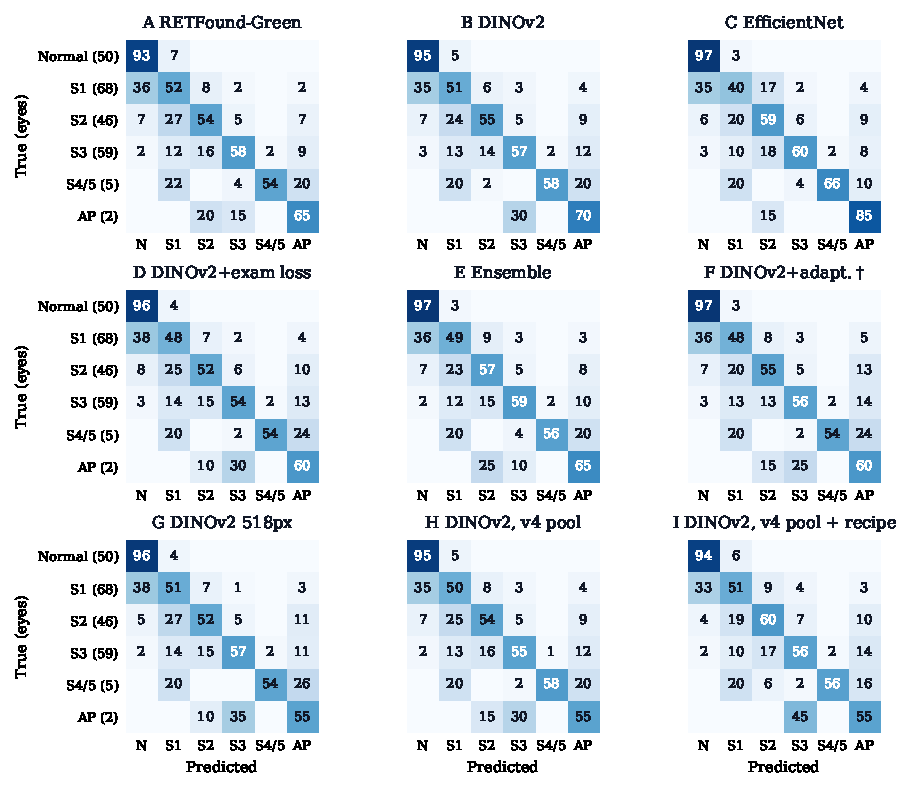
\includegraphics[width=0.8\textwidth]{fig_confusion_dev_eye.pdf}
\caption{Eye-level confusion matrices at the held-out cohort (development half), all nine arms. Cell: share of the true-class row in \%, averaged over each arm's \devLists{} models (diagonal = recall); blank = 0. True-class eye counts in parentheses. $^\dagger$Transductive.}
\label{fig:cm}
\end{figure*}

\begin{figure*}[!t]
\centering
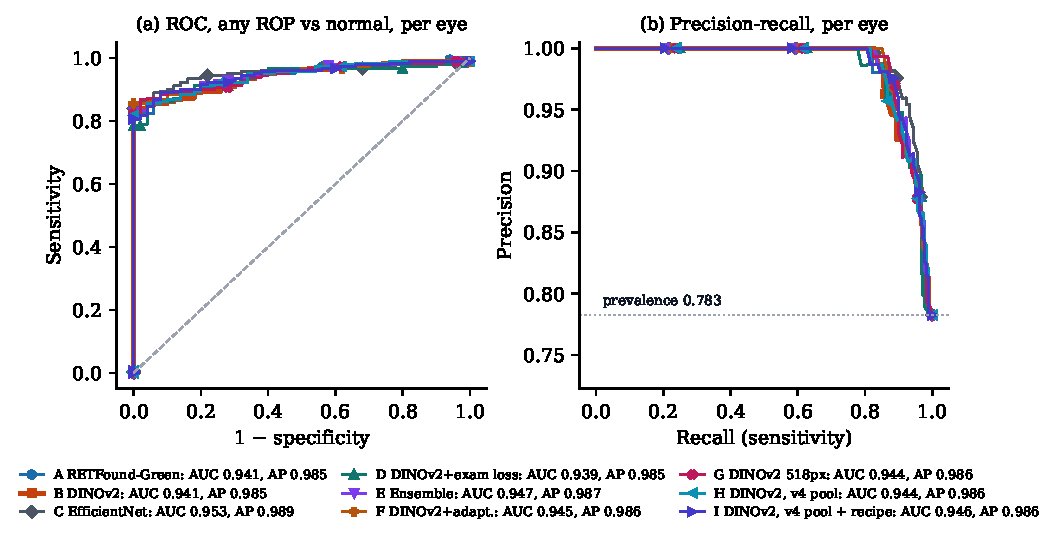
\includegraphics[width=\textwidth]{fig_roc_pr_dev_eye.pdf}
\caption{Any ROP vs normal per eye at the held-out cohort (development half), all arms: ROC and precision--recall, eye score averaged over each arm's \devLists{} models. Dotted: prevalence. Average precision is driven by the 78\% prevalence and is not informative here.}
\label{fig:roc}
\end{figure*}

\begin{figure*}[!t]
\centering
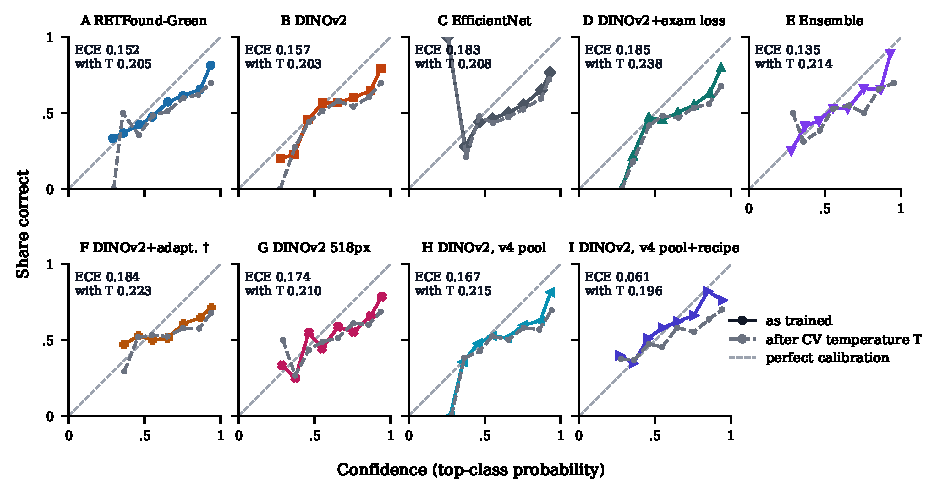
\includegraphics[width=\textwidth]{fig_reliability_dev_eye.pdf}
\caption{Reliability of the eye-level top-class probability at the held-out cohort, ten equal-width bins, seeds pooled: as trained (color) and after each seed's cross-validation temperature (gray). The temperature makes every arm more over-confident at the new site.}
\label{fig:reliability}
\end{figure*}

\begin{figure*}[!t]
\centering
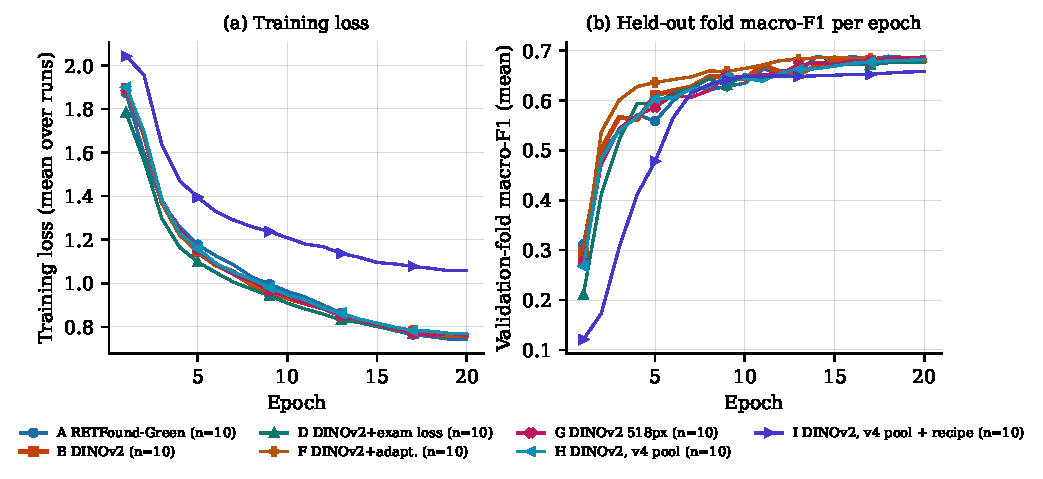
\includegraphics[width=\textwidth]{fig_training_curves.pdf}
\caption{Training curves, mean over each arm's \nRuns{} runs (five folds $\times$ two seeds): (a) training loss; (b) macro-F1 on the held-out fold per epoch.}
\label{fig:training}
\end{figure*}

\begin{figure*}[!t]
\centering
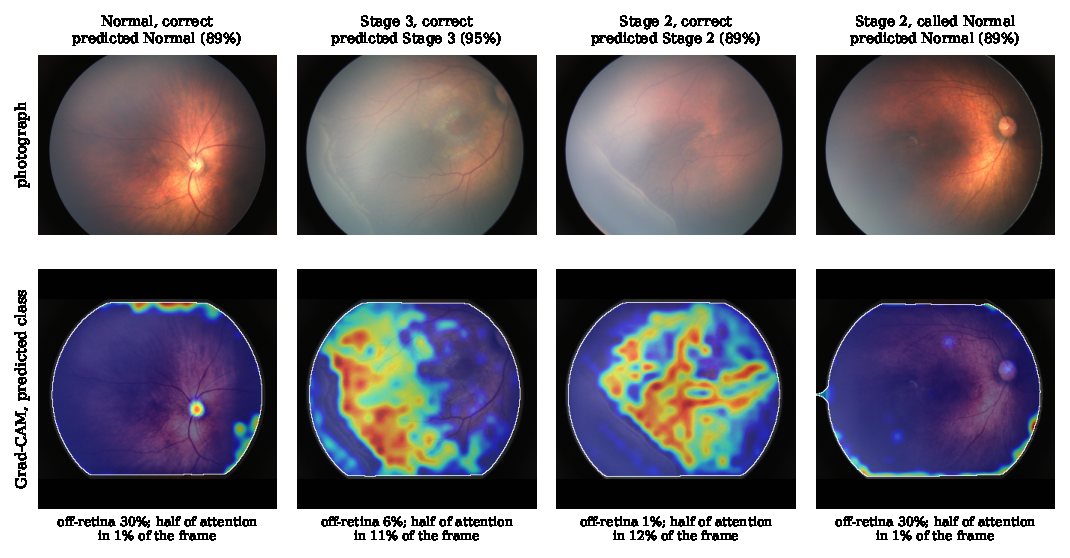
\includegraphics[width=\textwidth]{fig_gradcam.pdf}
\caption{Grad-CAM of the served ensemble (arm B, seed \seedA{}, five checkpoints) for development-half photographs, chosen by a fixed rule (the most confident example of each outcome: a correct normal, a correct stage 3, a correct stage 2, and a stage-2 photograph called normal). Maps are colored inside the retinal field only; under each, the share of attention outside the retina and how much of the frame holds half of it. Maps show what moved the score; they are not evidence of correctness and were not validated against ridge annotations.}
\label{fig:gradcam}
\end{figure*}

\section{Independent packages}
\begin{table}[!t]
\caption{Classical learners on \mateMLFeat{} hand-crafted features (independent package; four classes; photo-level 80/20 split; CV: five-fold accuracy on the augmented training rows, which ranked the learners; s: training seconds). Not comparable with the protocol results (main text, Sec.~IV-C).}
\label{tab:mateml}
\centering\scriptsize\setlength{\tabcolsep}{3pt}
\begin{tabular}{@{}lccccccr@{}}
\toprule
 & CV & \multicolumn{5}{c}{Test, 629 photographs} & \\
\cmidrule(lr){3-7}
Model & Acc. & Acc. & Bal.\,acc. & mF1 & QWK & AUC & s\\
\midrule
SVM (RBF) & 0.562 & 0.585 & 0.576 & 0.576 & 0.547 & 0.812 & 23 \\
Soft Voting (top-3) & 0.571 & 0.585 & 0.571 & 0.569 & 0.573 & 0.810 & 593 \\
Extra Trees & 0.542 & 0.574 & 0.561 & 0.555 & 0.502 & 0.790 & 6 \\
XGBoost & 0.562 & 0.568 & 0.554 & 0.552 & 0.535 & 0.804 & 130 \\
HistGradBoost & 0.566 & 0.568 & 0.552 & 0.550 & 0.551 & 0.807 & 459 \\
LightGBM & 0.567 & 0.566 & 0.555 & 0.555 & 0.563 & 0.810 & 39 \\
MLP & 0.534 & 0.558 & 0.547 & 0.549 & 0.531 & 0.795 & 13 \\
Stacking (top-3) & 0.567 & 0.556 & 0.543 & 0.541 & 0.556 & 0.807 & 2{,}107 \\
Random Forest & 0.540 & 0.555 & 0.540 & 0.532 & 0.500 & 0.786 & 9 \\
CatBoost & 0.547 & 0.522 & 0.511 & 0.508 & 0.458 & 0.784 & 33 \\
KNN & 0.518 & 0.501 & 0.493 & 0.489 & 0.403 & 0.736 & 5 \\
Logistic Reg. & 0.520 & 0.488 & 0.477 & 0.475 & 0.410 & 0.762 & 6 \\
\bottomrule
\end{tabular}

\end{table}

\begin{table}[!t]
\caption{Independent CNN package: ImageNet-pretrained CNNs (timm), 224~px, up to 40 epochs with early stopping on validation macro-F1; the soft vote averages the three with the highest validation macro-F1. Four classes; photo-level split.}
\label{tab:matecnn}
\centering\scriptsize\setlength{\tabcolsep}{1.9pt}
\begin{tabular}{@{}lccc@{\hspace{6pt}}ccccc@{}}
\toprule
 & & & Val & \multicolumn{5}{c}{Test, 315 photographs}\\
\cmidrule(l){5-9}
Model & Par.\,(M) & Ep. & mF1 & Acc. & Bal. & mF1 & QWK & AUC\\
\midrule
resnest50d & 25.4 & 32 & 0.821 & 0.835 & 0.827 & 0.828 & 0.898 & 0.956 \\
densenet121 & 7.0 & 36 & 0.822 & 0.822 & 0.816 & 0.815 & 0.880 & 0.942 \\
efficientnet\_b2 & 7.7 & 40 & 0.832 & 0.819 & 0.812 & 0.811 & 0.884 & 0.943 \\
resnet50 & 23.5 & 40 & 0.827 & 0.810 & 0.802 & 0.800 & 0.860 & 0.951 \\
mobilenetv3\_large\_100 & 4.2 & 22 & 0.769 & 0.775 & 0.775 & 0.769 & 0.840 & 0.925 \\
convnext\_tiny & 27.8 & 13 & 0.491 & 0.530 & 0.546 & 0.520 & 0.497 & 0.821 \\
\midrule
Soft vote, top 3 & -- & -- & 0.856 & 0.825 & 0.821 & 0.818 & 0.881 & 0.959 \\
\bottomrule
\end{tabular}

\end{table}

\begin{table*}[!t]
\caption{Independent foundation-model package: RETFound-DINOv2 ViT-L/14 frozen, LoRA adapters (rank 16, alpha 32 unless stated) on attention and MLP layers, linear four-class head; best epoch by validation macro-F1; four-view flip TTA. Probes: 10 epochs, one change each. Four classes; photo-level split.}
\label{tab:matefm}
\centering\scriptsize\setlength{\tabcolsep}{3.4pt}
\begin{tabular}{@{}l>{\raggedright\arraybackslash}p{3.3cm}ccc@{\hspace{5pt}}c@{\hspace{6pt}}ccccc@{}}
\toprule
 & & Trainable & & & Val & \multicolumn{5}{c}{Test, 315 photographs}\\
\cmidrule(l){7-11}
Run & Change & (M) & px & Epochs & mF1 & Acc. & Bal.\,acc. & mF1 & QWK & AUC\\
\midrule
\multicolumn{11}{@{}l}{\emph{Stage-2 probes, 10 epochs, seed 42 (one change each vs the first row)}}\\
p mlp & LoRA on attention + MLP (probe base) & 6.30 & 224 & 10 & 0.810 & 0.797 & 0.798 & 0.792 & 0.862 & 0.947 \\
p mlp r32 & rank 32, alpha 64 & 12.59 & 224 & 10 & 0.819 & 0.816 & 0.811 & 0.810 & 0.867 & 0.950 \\
p mlp dp1 & drop-path 0.1 & 6.30 & 224 & 10 & 0.830 & 0.797 & 0.799 & 0.793 & 0.861 & 0.951 \\
p mlp lr6e4 & lr 6e-4 & 6.30 & 224 & 10 & 0.829 & 0.829 & 0.825 & 0.823 & 0.897 & 0.958 \\
p mlp img280 & 280 px input & 6.30 & 280 & 10 & 0.834 & 0.822 & 0.821 & 0.818 & 0.875 & 0.959 \\
p mlp ord & ordinal auxiliary loss 0.3 & 6.30 & 224 & 10 & 0.807 & 0.806 & 0.807 & 0.803 & 0.876 & 0.951 \\
p mlp combo & r32 + dp 0.1 + lr 6e-4 + 280 px & 12.59 & 280 & 10 & 0.623 & 0.651 & 0.662 & 0.617 & 0.761 & 0.900 \\
\midrule
\multicolumn{11}{@{}l}{\emph{Full-length runs, 30 epochs max}}\\
final base s42 & attention-only LoRA, 30 ep & 2.37 & 224 & 30 & 0.817 & 0.825 & 0.818 & 0.818 & 0.900 & 0.956 \\
final mlp s42 & attention + MLP, 224 px, 30 ep & 6.30 & 224 & 25 & 0.816 & 0.778 & 0.763 & 0.765 & 0.860 & 0.948 \\
final mlp img280 s42 & chosen config, seed 42 & 6.30 & 280 & 25 & 0.846 & 0.787 & 0.787 & 0.779 & 0.870 & 0.950 \\
final mlp img280 s1 & chosen config, seed 1 & 6.30 & 280 & 30 & 0.841 & 0.822 & 0.818 & 0.815 & 0.888 & 0.952 \\
final mlp img280 s2 & chosen config, seed 2 & 6.30 & 280 & 30 & 0.846 & 0.832 & 0.827 & 0.826 & 0.889 & 0.951 \\
\midrule
3 seeds averaged & chosen config, seeds 42, 1, 2 & -- & -- & -- & 0.839 & 0.844 & 0.842 & 0.839 & 0.900 & 0.964 \\
3 seeds + 4 CNNs & plus EffNet-B2, ResNet50, DenseNet121, ResNeSt-50d & -- & -- & -- & 0.863 & 0.860 & 0.859 & 0.855 & 0.908 & 0.972 \\
\bottomrule
\end{tabular}

\end{table*}

\section{The served application}
\begin{figure*}[!t]
\centering
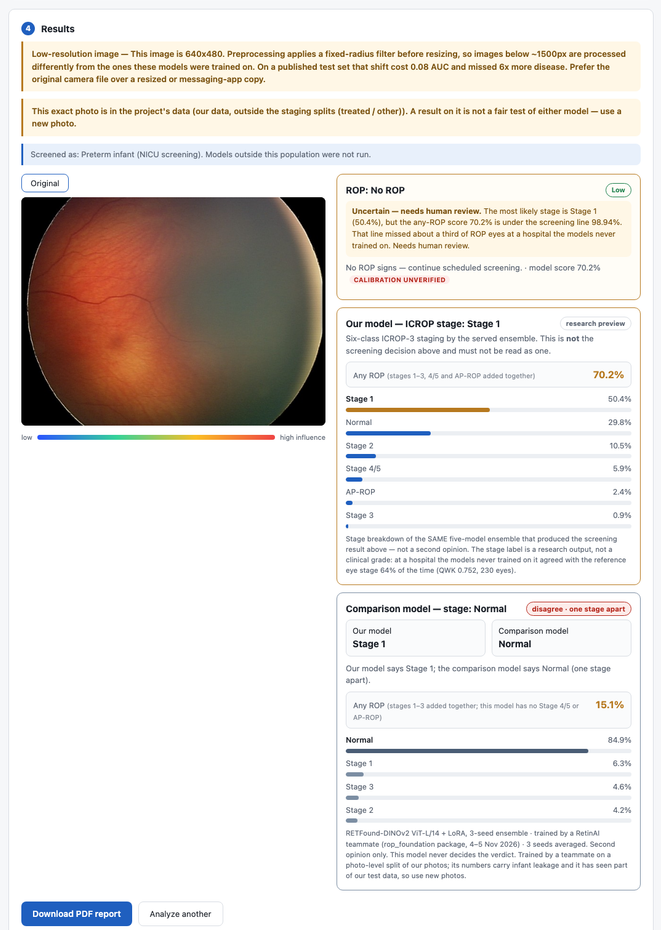
\includegraphics[width=0.92\textwidth]{fig_webapp.png}
\caption{The served application on a development-half photograph: verdict against the fixed operating point with the measured sensitivities, the served model's stage, the comparison model's stage with the agreement mark, and the seen-photo notice. Research prototype; not a medical device.}
\label{fig:webapp}
\end{figure*}

\section{Reporting checklist}
\begin{table*}[!t]
\caption{CLAIM 2024 items relevant to this study and where each is reported (main text unless stated). Items not applicable to a retrospective study of public data are omitted.}
\label{tab:claim}
\centering\scriptsize\setlength{\tabcolsep}{4pt}
\begin{tabular}{@{}>{\raggedright\arraybackslash}p{5.2cm}>{\raggedright\arraybackslash}p{11cm}@{}}
\toprule
Item & Where \\
\midrule
Study design, data sources, eligibility & Sec.~III-A (cascade, Fig.~1; Table~\ref{tab:funnel} here), Table~I \\
Reference standard, graders, label unit & Sec.~III-B and III-C: labels as released; grader counts not stated in the releases; exclusions from released diagnosis codes, not visual review \\
Demographics & Not available in the releases except ROP-VL (gestational age, birth weight), not used; stated in Sec.~III-A \\
Data partitions, leakage control & Sec.~III-D (patient-grouped folds, held-out cohort, duplicate exclusion), Sec.~III-E (audit, Table~II) \\
Preprocessing, augmentation & Sec.~III-F, Fig.~2 \\
Model architectures and training & Sec.~IV; Table~\ref{tab:recipe} here \\
Model selection rule, pre-specification & Sec.~IV-B (protocol commit and amendments, selection rule, margins) \\
Evaluation metrics, intervals, multiplicity & Sec.~IV-B and V-C (bootstrap over infants, paired contrasts, minimum detectable difference, Holm policy) \\
External evaluation & Sec.~V-C--V-E (held-out cohort, development half; locked half unscored for the transformers) \\
Calibration & Sec.~V-E; Fig.~\ref{fig:reliability} here \\
Failure analysis & Sec.~V-D (confusion by stage); Fig.~\ref{fig:gradcam} here (qualitative, not validated) \\
Limitations & Sec.~VI \\
Data, code, model availability & Data and Code Availability (repository, generator scripts, weight hashes) \\
AI-use disclosure & Acknowledgments \\
\bottomrule
\end{tabular}
\end{table*}

\end{document}
